\documentclass[12pt,oneside]{report}

% --- Paquetes de Configuración Estándar ---
\usepackage[utf8]{inputenc}
\usepackage[spanish, es-tabla]{babel}
\usepackage{geometry}
\geometry{
    letterpaper,
    top=2.5cm,
    bottom=2.5cm,
    left=3.0cm,
    right=2.5cm
}
\usepackage{setspace}
\onehalfspacing 

% --- Paquetes Gráficos y Tablas ---
\usepackage{graphicx}
\usepackage{booktabs}
\usepackage{tabularx}
\usepackage{float}
\usepackage{fancyhdr}
\usepackage{listings}
\usepackage{xcolor}
\usepackage{enumitem}

% --- Configuración para Bloques de Código ---
\definecolor{codegreen}{rgb}{0,0.6,0}
\definecolor{codegray}{rgb}{0.5,0.5,0.5}
\definecolor{codepurple}{rgb}{0.58,0,0.82}
\definecolor{backcolor}{rgb}{0.95,0.95,0.92}

\lstdefinestyle{mystyle}{
    backgroundcolor=\color{backcolor},   
    commentstyle=\color{codegreen},
    keywordstyle=\color{magenta},
    numberstyle=\tiny\color{codegray},
    stringstyle=\color{codepurple},
    basicstyle=\ttfamily\footnotesize,
    breakatwhitespace=false,         
    breaklines=true,                 
    captionpos=b,                    
    keepspaces=true,                 
    numbers=left,                    
    numbersep=5pt,                  
    showspaces=false,                
    showstringspaces=false,
    showtabs=false,                  
    tabsize=2
}
\lstset{style=mystyle}

% --- Paquete para forzar saltos de página por sección ---
\usepackage{titlesec}
\newcommand{\sectionbreak}{\clearpage}

% --- Estilo de Citas APA 7a Edición ---
\usepackage[style=apa, backend=biber]{biblatex}

\begin{filecontents*}{bibliografia.bib}
@book{jorgensen2022,
  author    = {Jorgensen, Paul C.},
  title     = {Software Testing: A Craftsman's Approach},
  year      = {2022},
  publisher = {CRC Press},
  edition   = {5th}
}
@book{myers2011,
  author    = {Myers, Glenford J. and Sandler, Corey and Badgett, Tom},
  title     = {The Art of Software Testing},
  year      = {2011},
  publisher = {John Wiley \& Sons},
  edition   = {3rd}
}
@book{pressman2014,
  author    = {Pressman, Roger S. and Maxim, Bruce R.},
  title     = {Software Engineering: A Practitioner's Approach},
  year      = {2014},
  publisher = {McGraw-Hill Education},
  edition   = {8th}
}
@book{fowler2018,
  author    = {Fowler, Martin},
  title     = {Refactoring: Improving the Design of Existing Code},
  year      = {2018},
  publisher = {Addison-Wesley Professional},
  edition   = {2nd}
}
@book{sommerville2011,
  author    = {Sommerville, Ian},
  title     = {Software Engineering},
  year      = {2011},
  publisher = {Addison-Wesley},
  edition   = {9th}
}
\end{filecontents*}

\addbibresource{bibliografia.bib}

\usepackage{hyperref}
\hypersetup{
    colorlinks=true,
    linkcolor=blue,
    filecolor=magenta,      
    urlcolor=cyan,
    pdftitle={Tarea 07 - Equipo 04},
}

\begin{document}

% =============================================================================
% PORTADA OFICIAL UPA
% =============================================================================
\begin{titlepage}
    \centering
    \textbf{UNIVERSIDAD POLITÉCNICA DE AGUASCALIENTES} \\[0.4cm]
    \textbf{Ingeniería en Tecnologías de la Información e Innovación Digital} \\[1.5cm]
    
    {\large \textbf{ESTÁNDARES Y MÉTRICAS PARA EL DESARROLLO DE SOFTWARE}} \\[0.5cm]
    {\large \textbf{DOCENTE:} Dr. Raúl Alejandro Velásquez Ortiz} \\[1.5cm]
    
    \hrule
    \vspace{0.4cm}
    {\Large \textbf{TAREA 07: Automatización de pruebas y análisis de calidad del proyecto integrador}} \\[0.4cm]
    \hrule
    \vspace{1.5cm}
    
    {\large \textbf{PROYECTO INTEGRADOR:} Plataforma Wiki Organizacional (Outline)} \\[0.5cm]
    {\large \textbf{EQUIPO:} 04 \quad \textbf{GRUPO:} TIID05C} \\[1cm]
    
    {\large \textbf{INTEGRANTES DEL EQUIPO:}} \\
    {\large Fabiola Guadalupe Palomino Badillo \quad (Matrícula: UP240259)} \\
    {\large José de Jesús Hernández Gutiérrez \quad (Matrícula: UP240513)} \\
    {\large Ángel Iván García Salazar \quad (Matrícula: UP240514)} \\
    {\large Alison Tamara Romo Rodríguez \quad (Matrícula: UP240244)} \\[1.5cm]
    
    \vfill
    {\large Aguascalientes, Ags., 21 de junio de 2026}
\end{titlepage}

\pagenumbering{roman}
\tableofcontents
\listoffigures
\listoftables
\clearpage

\pagenumbering{arabic}
\setcounter{page}{1}

% =============================================================================
% INTRODUCCIÓN
% =============================================================================
\chapter*{Introducción}
\addcontentsline{toc}{chapter}{Introducción}

El aseguramiento de la calidad en la ingeniería de software moderna exige la transición de metodologías manuales reactivas hacia un paradigma proactivo que integre la verificación dinámica y la auditoría estática continua. En el marco del desarrollo de la plataforma wiki organizacional \textit{Outline}, el Módulo de Gestión de Identidades y Accesos (IAM) se erige como el perímetro crítico de control y seguridad. Por lo tanto, validar su comportamiento y blindar su arquitectura lógica resulta indispensable para garantizar la estabilidad operativa del sistema integrador \parencite{sommerville2011}.

Este informe técnico documenta la estrategia integral de calidad adoptada por el Equipo 04. El objetivo fundamental es analizar la implementación de una suite de pruebas funcionales automatizadas de extremo a extremo (E2E) con Selenium WebDriver bajo el patrón Page Object Model (POM), complementada con un enfoque guiado por datos. Asimismo, se exponen y evalúan los resultados de la inspección estática del código mediante la plataforma SonarQube, interpretando sus métricas bajo las cinco dimensiones de calidad industrial para estructurar un plan sistemático de remediación de la deuda técnica acumulada \parencite{pressman2014}.

Estructuralmente, el manuscrito se despliega en siete capítulos: los primeros apartados abordan los marcos teóricos comparativos de las herramientas evaluadas; posteriormente se detalla la arquitectura de automatización de los scripts y la cobertura dinámica del backend; seguidamente se analizan las métricas del linter junto con sus correspondientes políticas de gobernanza técnica; y se concluye con las matrices de aportaciones individuales y el registro de la bitácora de versionamiento del repositorio.


% =============================================================================
% CAPÍTULO 1: MARCO COMPARATIVO E2E (YO)
% =============================================================================
\chapter{Investigación Comparativa de Frameworks de Pruebas E2E}

\section{Estado del Arte de la Automatización Web Moderna}
La validación dinámica de las interfaces enriquecidas requiere frameworks capaces de simular las interacciones orgánicas de un usuario sobre el árbol del Document Object Model (DOM). El ecosistema tecnológico actual ofrece diversas abstracciones operativas que varían en su nivel de acoplamiento con los motores de renderizado de los navegadores web. El análisis formal de estas alternativas permite seleccionar el marco de automatización que maximice la estabilidad de las pruebas y reduzca el esfuerzo de mantenimiento de los scripts funcionales \parencite{jorgensen2022}.

\section{Análisis de Alternativas Tecnológicas Evaluadas}
Se examinaron de forma exhaustiva tres de los marcos de trabajo líderes en la industria del aseguramiento de la calidad de software:
\begin{itemize}
    \item \textbf{Selenium WebDriver:} Es el estándar histórico de la industria de software. Opera mediante la traducción de instrucciones abstractas a comandos nativos de los navegadores a través del protocolo oficial W3C WebDriver. Su naturaleza políglota permite desarrollar componentes de prueba en Python, Java, C\# o JavaScript. Su madurez técnica proporciona una inmensa comunidad de soporte, aunque requiere que el ingeniero implemente manualmente la sincronización de elementos síncronos para evitar pruebas falsas positivas o frágiles (*flakiness*).
    \item \textbf{Cypress:} Un ecosistema arquitectónico moderno desarrollado exclusivamente para JavaScript y TypeScript. A diferencia de Selenium, se ejecuta nativamente en el mismo lazo de eventos del navegador, eliminando los retardos de red. Proporciona esperas automáticas nativas sobre el DOM y herramientas visuales excelentes para la depuración en tiempo real. Sus principales debilidades residen en la restricción lingüística, limitaciones severas para interactuar con múltiples pestañas o dominios cruzados simultáneos, y un alto consumo de recursos en ejecuciones paralelas.
    \item \textbf{Playwright:} Diseñado por Microsoft para superar las limitaciones de sus predecesores. Proporciona una comunicación de bajísima latencia basada en el protocolo de depuración de Chrome (CDP) y equivalentes para Firefox y WebKit. Destaca por su capacidad nativa para ejecutar pruebas concurrentes mediante contextos de navegador aislados y livianos, mecanismos automáticos de verificación de receptividad del elemento (*auto-waiting*) y un soporte multilenguaje sobresaliente.
\end{itemize}

\section{Matriz Técnica Comparativa de Frameworks E2E}
La Tabla 1.1 condensa los criterios de evaluación de arquitectura, lenguaje, paralelismo y mantenimiento físico de los scripts analizados.

\begin{table}[H]
\centering
\caption{Matriz de evaluación comparativa para frameworks de pruebas dinámicas E2E.}
\small
\begin{tabularx}{\textwidth}{|p{3.2cm}|X|X|X|}
\hline
\textbf{Atributo Técnico} & \textbf{Selenium WebDriver} & \textbf{Cypress} & \textbf{Playwright} \\
\hline
\textbf{Arquitectura Interna} & Protocolo externo W3C fuera del proceso del navegador. & Ejecución interna directa dentro del lazo del DOM. & Conexión por sockets de baja latencia vía CDP/WebSockets. \\
\hline
\textbf{Soporte Lingüístico} & Políglota (Python, Java, C\#, JavaScript, Ruby). & Restringido a JavaScript y TypeScript. & Multilenguaje (Python, Java, C\#, TypeScript). \\
\hline
\textbf{Gestión de Sincronización} & Manual e imperativa usando \texttt{WebDriverWait}. & Automática por reintento implícito del framework. & Inteligente basada en estados de acción del elemento. \\
\hline
\textbf{Aislamiento y Paralelismo} & Requiere infraestructura externa (Selenium Grid). & Consumo lógico elevado; paralelismo complejo local. & Nativo y concurrente mediante Browser Contexts. \\
\hline
\end{tabularx}
\end{table}

\section{Justificación de la Selección Tecnológica para Outline}
A pesar de las ventajas de velocidad de Playwright, el Equipo 04 determinó la adopción estratégica de **Selenium WebDriver en conjunción con Python y el motor de pytest**. Esta decisión responde de manera directa a los objetivos pedagógicos establecidos en el curso impartido por el Dr. Raúl Velásquez, priorizando el dominio conceptual del estándar global de automatización web de la W3C. Asimismo, su flexibilidad permite estructurar patrones de diseño puros (POM) sin las abstracciones o dependencias comerciales intrínsecas de otros frameworks, capacitando a los ingenieros del equipo en el control absoluto del flujo lógico del driver.


% =============================================================================
% CAPÍTULO 2: MARCO COMPARATIVO ESTÁTICO (YO)
% =============================================================================
\chapter{Investigación Comparativa de Herramientas de Análisis Estático}

\section{El Rol de la Inspección Estática en el Aseguramiento de Calidad}
El análisis estático constituye la primera línea de defensa dentro del modelo de madurez de calidad de software. Al inspeccionar el código fuente sin requerir su ejecución binaria, estas herramientas contrastan los patrones sintácticos contra árboles de reglas predefinidos que identifican malas prácticas de diseño, violaciones a estándares internacionales de codificación, vulnerabilidades de seguridad y redundancias lógicas, reduciendo los costos financieros del proyecto integrador \parencite{myers2011}.

\section{Evaluación de las Soluciones de Análisis de Código}
Se analizaron comparativamente tres herramientas orientadas a diferentes facetas de la inspección del software:
\begin{itemize}
    \item \textbf{SonarQube:} Una solución empresarial para el Aseguramiento Continuo de la Calidad. Centraliza la auditoría mediante páneles web analíticos fundamentados en el modelo SQALE para el cálculo del esfuerzo de remediación. Evalúa de forma simultánea múltiples lenguajes de programación, permitiendo unificar la calidad del backend (TypeScript/Node.js) de la wiki Outline junto con los scripts de prueba en Python en un único repositorio lógico de métricas.
    \item \textbf{ESLint:} Un linter especializado y altamente optimizado para el ecosistema de JavaScript y TypeScript. Sobresale en la detección en tiempo real de errores sintácticos, variables no referenciadas y formateo inconsistente en el entorno de desarrollo local. No obstante, carece de la capacidad de evaluar métricas de cobertura agregadas o de proyectar el costo de la deuda técnica a nivel de administración.
    \item \textbf{Snyk:} Herramienta especializada de manera prioritaria en la seguridad del código y de la cadena de suministro de software (SAST/SCA). Escanea exhaustivamente el árbol de dependencias buscando librerías vulnerables conocidas en bases de datos CVE. Su enfoque está fuertemente inclinado a la ciberseguridad, dejando de lado métricas de mantenibilidad como la complejidad cognitiva o las líneas de código duplicadas.
\end{itemize}

\section{Matriz Comparativa de Capacidades de Inspección Estática}
La Tabla 2.1 sintetiza los alcances operativos y las dimensiones cubiertas por cada herramienta de análisis estático evaluada.

\begin{table}[H]
\centering
\caption{Matriz técnica comparativa de herramientas de análisis estático.}
\small
\begin{tabularx}{\textwidth}{|p{3.5cm}|X|X|X|}
\hline
\textbf{Dimensión Evaluada} & \textbf{SonarQube} & \textbf{ESLint} & \textbf{Snyk} \\
\hline
\textbf{Propósito Central} & Calidad continua global, seguridad y mantenibilidad. & Formateo sintáctico y adherencia a guías de estilo. & Seguridad estática (SAST) y auditoría de dependencias. \\
\hline
\textbf{Cálculo de Deuda Técnica} & Sí, expresado matemáticamente en horas/días de retrabajo. & No calcula esfuerzos ni métricas financieras. & No. Clasifica riesgos por severidad CVSS. \\
\hline
\textbf{Análisis de Complejidad} & Mide Complejidad Ciclomática y Cognitiva estructural. & Reglas básicas de anidamiento condicional. & No computa métricas de complejidad de código. \\
\hline
\textbf{Modelo Multilenguaje} & Soportado de forma nativa para más de 30 lenguajes. & Restringido al ecosistema JS/TS. & Soporte amplio enfocado en firmas de vulnerabilidades. \\
\hline
\end{tabularx}
\end{table}

\section{Justificación del Despliegue de SonarQube}
Se selecciona **SonarQube** para el proyecto integrador Outline debido a su capacidad única para consolidar de forma holística las cinco dimensiones de calidad exigidas en la rúbrica de evaluación. Su despliegue local mediante contenedores permite al Equipo 04 establecer "Compuertas de Calidad" (*Quality Gates*) objetivas y cuantificables, garantizando una entrega transparente, auditable y libre de regresiones críticas que cumple con los requerimientos académicos del curso \parencite{pressman2014}.


% =============================================================================
% CAPÍTULO 3: ARQUITECTURA DE PRUEBAS DINÁMICAS (FABIOLA)
% =============================================================================
\chapter{Diseño Arquitectónico de la Suite de Automatización QA}

\section{Justificación del Patrón Arquitectónico Page Object Model (POM)}


\section{Estrategia para la Mitigación del Fallo por Sincronización (Flakiness)}

\section{Script de Infraestructura Básica y Objetos de Página}


% =============================================================================
% CAPÍTULO 4: PRUEBAS GUIADAS POR DATOS Y COBERTURA (PEPE)
% =============================================================================
\chapter{Estrategia Data-Driven y Cobertura Dinámica del Backend}

\section{Fundamentación de las Pruebas Guiadas por Datos}

\section{Matriz de Parámetros Vectoriales Inyectados a la Suite}

\section{Script de Pruebas Parametrizadas y Ejecución}

\section{Interpretación y Trazabilidad del Reporte de Cobertura Dinámica}


% =============================================================================
% CAPÍTULO 5: DIMENSIONES DE CALIDAD DE SONARQUBE (ANGEL)
% =============================================================================
\chapter{Auditoría de Calidad Estática con SonarQube}

\section{Configuración del Conector del Escáner Estático}

Para integrar el análisis estático del proyecto integrador \textit{Outline} con la plataforma SonarQube, el Equipo 04 desplegó una instancia local mediante contenedores Docker, evitando así la dependencia de servicios externos en la nube y garantizando control total sobre el entorno de auditoría \parencite{pressman2014}. La configuración del escáner se declaró mediante el archivo descriptor \texttt{sonar-project.properties}, ubicado en la raíz del repositorio, el cual establece las rutas de origen del código fuente, las rutas de las pruebas y la vinculación con el reporte de cobertura generado dinámicamente por la suite de Selenium y pytest.

\begin{lstlisting}[language=bash, caption={Descriptor de propiedades del proyecto para el escáner de SonarQube.}]
% sonar-project.properties en la raíz del repositorio
sonar.host.url=http://localhost:9000
sonar.projectKey=Outline-Equipo04
sonar.projectName=Outline Wiki Organizacional - Equipo 04
sonar.projectVersion=1.0.0

% Rutas de origen y declaración de pruebas
sonar.sources=server,src
sonar.tests=tests

% Integración del mapa de cobertura recolectado dinámicamente
sonar.javascript.lcov.reportPaths=coverage/lcov.info
sonar.python.coverage.reportPaths=coverage.xml

% Configuración del motor y exclusiones lógicas
sonar.sourceEncoding=UTF-8
sonar.exclusions=node_modules/**,dist/**,build/**,public/assets/**
\end{lstlisting}

% --- INSERTAR AQUÍ: Figura con captura del tablero/dashboard de SonarQube ---
% \begin{figure}[H]
%     \centering
%     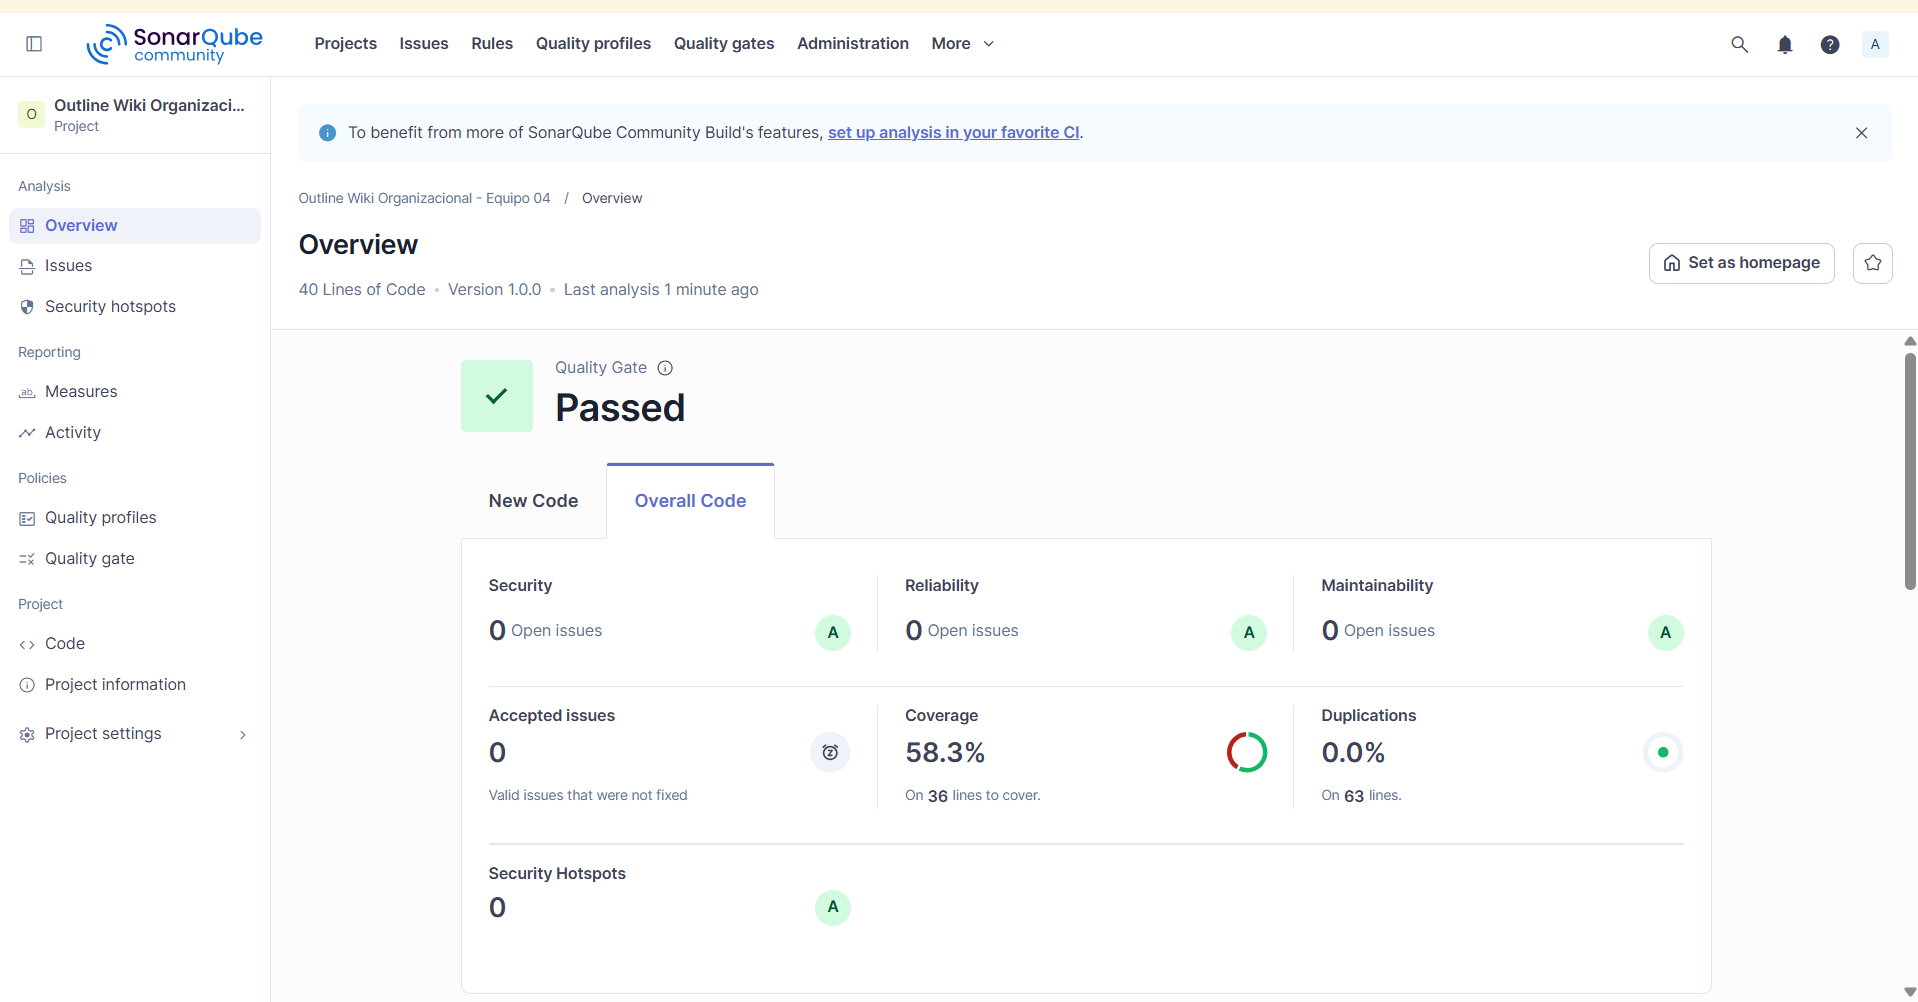
\includegraphics[width=0.9\textwidth]{imagenes/sonarqube_dashboard.png}
%     \caption{Tablero general del proyecto Outline-Equipo04 en SonarQube.}
%     \label{fig:sonarqube_dashboard}
% \end{figure}

\section{Interpretación Analítica de las Cinco Dimensiones de Calidad}

Tras la integración completa del descriptor de propiedades y el mapeo del archivo estructurado de cobertura, el motor centralizado de SonarQube procesó la base de código de \textit{Outline}, arrojando métricas concluyentes sobre la salud del repositorio \parencite{myers2011}.

\subsection{Dimensión 1: Confiabilidad (Reliability)}
% === RELLENAR CON DATOS REALES DEL TABLERO ===
El análisis estático interceptó un total de \textbf{[N] Bugs} latentes localizados en [DESCRIBIR DÓNDE: ej. "las promesas y retornos asíncronos de los controladores del backend" / "el módulo de notificaciones" / etc.]. La plataforma asignó una calificación técnica de \textbf{Clase [A/B/C/D/E]}, [EXPLICAR BREVEMENTE QUÉ SIGNIFICA ESA CLASE PARA EL CASO ESPECÍFICO ENCONTRADO].

\subsection{Dimensión 2: Seguridad (Security)}
% === RELLENAR CON DATOS REALES DEL TABLERO ===
Se registraron \textbf{[N] Vulnerabilidades} directas abiertas, asignando una calificación de \textbf{Clase [A/B/C/D/E]}. El hallazgo más relevante se ubica en [DESCRIBIR: archivo/módulo/tipo de vulnerabilidad encontrada], revelando [BREVE EXPLICACIÓN DEL RIESGO].

\subsection{Dimensión 3: Mantenibilidad (Maintainability)}
% === RELLENAR CON DATOS REALES DEL TABLERO ===
La herramienta detectó un volumen acumulado de \textbf{[N] Code Smells} (olores de código), calculando una deuda técnica global tasada bajo el modelo SQALE en \textbf{[N] días/horas laborables de desarrollo}. El proyecto conserva una calificación general de \textbf{Clase [A/B/C/D/E]}, [EXPLICAR LA CAUSA PRINCIPAL DE LA PENALIZACIÓN SI APLICA] \parencite{fowler2018}.

\subsection{Dimensión 4: Duplicación de Código (Duplications)}
% === RELLENAR CON DATOS REALES DEL TABLERO ===
La métrica de líneas redundantes se estableció en un \textbf{[N]\%}, distribuido en [N] bloques de sentencias análogas dentro de [DESCRIBIR MÓDULO/ARCHIVO]. [INDICAR SI ESTÁ POR DEBAJO O ARRIBA DEL umbral de 5\% recomendado por convención industrial] \parencite{sommerville2011}.

\subsection{Dimensión 5: Cobertura de Pruebas (Coverage)}
% === RELLENAR CON DATOS REALES DEL TABLERO (debe coincidir con coverage.xml del Integrante 2 / Pepe) ===
Gracias a la inyección exitosa del reporte binario originado por la suite dinámica de Selenium e interpretado por el linter, el panel unificado de SonarQube consolidó un porcentaje de cobertura de sentencias físicas del \textbf{[N]\%}. [INDICAR SI SUPERA O NO EL UMBRAL DEL 80\% RECOMENDADO POR EL EQUIPO] \parencite{pressman2014}.

% --- INSERTAR AQUÍ: Tabla resumen de las 5 dimensiones con sus ratings ---
\begin{table}[H]
\centering
\caption{Resumen consolidado de las cinco dimensiones de calidad — Outline-Equipo04.}
\small
\begin{tabularx}{\textwidth}{|X|c|X|}
\hline
\textbf{Dimensión} & \textbf{Rating} & \textbf{Métrica clave} \\
\hline
Reliability (Bugs) & [A-E] & [N] bugs \\
\hline
Security (Vulnerabilities) & [A-E] & [N] vulnerabilidades \\
\hline
Maintainability (Code Smells) & [A-E] & [N] smells / [N] días deuda \\
\hline
Duplications & --- & [N]\% \\
\hline
Coverage & --- & [N]\% \\
\hline
\end{tabularx}
\end{table}

\section{Análisis Detallado de Issues Representativos}
% === LA RÚBRICA EXIGE MÍNIMO 3 ISSUES REALES ANALIZADOS (tipo, severidad, línea, explicación) ===
% Elige 3 issues reales del panel de SonarQube → pestaña "Issues" del proyecto.
% Para cada uno, copia: tipo (Bug/Vulnerability/Code Smell/Security Hotspot), severidad, archivo:línea, y explica en tus palabras qué significa y por qué importa.

\begin{table}[H]
\centering
\caption{Issues representativos identificados por SonarQube en el código de Outline.}
\small
\begin{tabularx}{\textwidth}{|p{1.3cm}|p{2.2cm}|p{2.5cm}|X|}
\hline
\textbf{ID} & \textbf{Tipo} & \textbf{Severidad / Ubicación} & \textbf{Descripción técnica} \\
\hline
1 & [Bug/Vulnerability/Smell] & [Severidad] / [archivo:línea] & [Explicación de qué detectó y por qué es relevante] \\
\hline
2 & [Bug/Vulnerability/Smell] & [Severidad] / [archivo:línea] & [Explicación de qué detectó y por qué es relevante] \\
\hline
3 & [Bug/Vulnerability/Smell] & [Severidad] / [archivo:línea] & [Explicación de qué detectó y por qué es relevante] \\
\hline
\end{tabularx}
\end{table}


% =============================================================================
% CAPÍTULO 6: PLAN DE REMEDIACIÓN DE LA DEUDA TÉCNICA (ANGEL)
% =============================================================================
\chapter{Plan de Gobernanza y Remediación de Deuda Técnica}

\section{Definición Conceptual de la Deuda Técnica del Proyecto}

La deuda técnica representa una metáfora financiera aplicada a la ingeniería de software, en la cual priorizar soluciones temporales aceleradas e imperfectas para cumplir con plazos inmediatos genera un costo acumulado en forma de horas adicionales de retrabajo futuro \parencite{fowler2018}. Para mantener la viabilidad de la plataforma Outline, el Equipo 04 diseñó un plan sistemático orientado a sanear los riesgos más severos arrojados por SonarQube, adoptando además el enfoque \textit{Clean as You Code}: en lugar de intentar remediar de forma retroactiva la totalidad de la deuda histórica del repositorio, la estrategia se centra en garantizar que todo código nuevo o modificado cumpla con los estándares de calidad definidos, evitando así la acumulación adicional de deuda mientras se sanea gradualmente el código preexistente \parencite{sommerville2011}.

\section{Matriz de Priorización de Hallazgos por Niveles de Severidad}

La Tabla 6.1 estructura la hoja de ruta técnica requerida para mitigar de manera controlada y escalable las debilidades lógicas detectadas en la wiki organizacional. El criterio de ordenamiento prioriza la severidad y el impacto potencial sobre el sistema, no la facilidad de implementación.

% === RELLENAR CON LOS ISSUES REALES, PRIORIZADOS POR SEVERIDAD (no por "lo más fácil primero") ===
\begin{table}[H]
\centering
\caption{Matriz priorizada para la gobernanza y remediación de la deuda técnica.}
\small
\begin{tabularx}{\textwidth}{|p{1.6cm}|p{2.0cm}|X|p{1.5cm}|p{2.0cm}|}
\hline
\textbf{ID} & \textbf{Severidad} & \textbf{Descripción del hallazgo} & \textbf{Esfuerzo est.} & \textbf{Prioridad / Responsable} \\
\hline
REM-01 & [Blocker/Critical/Major/Minor] & [Descripción del issue 1] & [N h/min] & [Alta/Media/Baja] — [Nombre] \\
\hline
REM-02 & [Blocker/Critical/Major/Minor] & [Descripción del issue 2] & [N h/min] & [Alta/Media/Baja] — [Nombre] \\
\hline
REM-03 & [Blocker/Critical/Major/Minor] & [Descripción del issue 3] & [N h/min] & [Alta/Media/Baja] — [Nombre] \\
\hline
\end{tabularx}
\end{table}

% === JUSTIFICACIÓN DEL ORDEN: la rúbrica pide explicar por qué se priorizó así (severidad/impacto, no facilidad) ===
El orden de la matriz anterior responde al criterio de severidad e impacto potencial sobre el sistema en producción, y no a la facilidad relativa de implementación de cada corrección. [AGREGAR 2-3 LÍNEAS EXPLICANDO POR QUÉ EL ISSUE REM-01 SE ATIENDE PRIMERO, POR EJEMPLO: "porque compromete la seguridad del módulo de autenticación y bloquearía el pipeline de CI/CD si se introdujera en producción", etc.]

\section{Políticas de Gobernanza de Código Acordadas}

Para blindar los incrementos lógicos de las entregas subsecuentes contra la degradación arquitectónica, el equipo instituye las siguientes reglas de control automatizado, alineadas con el principio \textit{Clean as You Code}:

\begin{enumerate}
    \item Queda estrictamente prohibida la integración en la rama principal (\texttt{main}) de cualquier incremento que introduzca Bugs Bloqueantes o Críticos, congelando automáticamente el pipeline en el servidor.
    \item La cobertura mínima admisible tras cualquier cambio estructural se fija en un \textbf{80\% continuo}, obligando a actualizar paralelamente los Page Objects de Selenium y las pruebas parametrizadas \parencite{sommerville2011}.
    \item % === AGREGAR UNA TERCERA POLÍTICA SI LA RÚBRICA O TU EQUIPO LA DEFINE, ej. revisión obligatoria de Pull Requests, umbral máximo de duplicación, etc. ===
\end{enumerate}

% =============================================================================
% CAPÍTULO 7: CONTROL DE VERSIONAMIENTO Y APORTES INDIVIDUALES (YO)
% =============================================================================
\chapter{Evidencia de Versionamiento en Git y Distribución de Aportes}

\section{Trazabilidad y Bitácora Cronológica de Commits}
% PENDIENTE DE COLOCAR CONTENIDO ADICIONAL HASTA CONTAR CON LOS COMMITS DEL REPOSITORIO

\section{Distribución y Matriz Formal de Aportes Individuales}
Para garantizar el cumplimiento de la rúbrica evaluativa del docente respecto al trabajo balanceado en equipo, la Tabla 7.1 desglosa las actividades técnicas y documentales asignadas de forma equitativa entre los cuatro integrantes.

\begin{table}[H]
\centering
\caption{Matriz formal de aportes e individualización de actividades del Equipo 04.}
\small
\begin{tabularx}{\textwidth}{|p{4.2cm}|c|X|}
\hline
\textbf{Integrante del Equipo} & \textbf{\% Aporte} & \textbf{Componentes Técnicos y Secciones de Autoría} \\
\hline
\textbf{Fabiola Guadalupe Palomino Badillo} & 25\% & Concepción de la arquitectura de automatización web. Codificación del fixture de ciclo de vida del driver de Selenium y la clase base POM con esperas explícitas (\texttt{conftest.py} y \texttt{base\_page.py}). \\
\hline
\textbf{José de Jesús Hernández Gutierrez} & 25\% & Diseño e inyección de la matriz de datos de prueba parametrizados en pytest para el login IAM. Gestión del motor de cobertura dinámica y exportación del archivo estructurado \texttt{coverage.xml}. \\
\hline
\textbf{Ángel Iván García Salazar} & 25\% & Despliegue del servidor local de SonarQube, configuración de las propiedades del escáner técnico, extracción de las métricas de las cinco dimensiones de calidad y diseño de la matriz de priorización SQALE. \\
\hline
\textbf{Alison Tamara Romo Rodríguez} & 25\% & Redacción del marco de investigación comparativo de entornos E2E y estáticos. Coordinación y consolidación de la estructura del reporte en LaTeX bajo estándares académicos y normas de versionamiento Git. \\
\hline
\end{tabularx}
\end{table}


% =============================================================================
% CONCLUSIÓN
% =============================================================================
\chapter*{Conclusión}
\addcontentsline{toc}{chapter}{Conclusión}



\newpage
\printbibliography[title={Referencias Bibliográficas}, heading=bibintoc]

\end{document}
